\documentclass[tikz, border=8pt]{standalone}
\usepackage[T1]{fontenc}
\usepackage{tgpagella}
\usepackage{mathpazo}
\usepackage{tikz}
\usepackage{amsmath}
\usepackage{xcolor}
\usepackage{fontawesome5}
\usetikzlibrary{arrows.meta, shapes.geometric, calc, positioning}

% --- module palette (mirrors architecture.tex) ---
\definecolor{cEncB}{HTML}{2D8294}
\definecolor{cAdp}{HTML}{F0DFC9}
\definecolor{cAdpB}{HTML}{B07849}
\definecolor{cLLM}{HTML}{F4E6D5}
\definecolor{cLLMB}{HTML}{A0763C}
\definecolor{cPrompt}{HTML}{F1ECE3}
\definecolor{cPromptB}{HTML}{8E7A55}
\definecolor{cTok}{HTML}{E5EEF0}
\definecolor{cTokB}{HTML}{5E8090}
\definecolor{cBound}{HTML}{ECDFD3}
\definecolor{cBoundB}{HTML}{9C7558}
\definecolor{cAuT}{HTML}{F6E1CF}
\definecolor{cAuTB}{HTML}{C77F45}
% --- one colour per token type ---
\definecolor{cIns}{HTML}{F7CBA8}   \definecolor{cInsB}{HTML}{C77F45}
\definecolor{cCtx}{HTML}{F3DFA6}   \definecolor{cCtxB}{HTML}{C0952F}
\definecolor{cSpc}{HTML}{BCDBE2}   \definecolor{cSpcB}{HTML}{2D8294}
\definecolor{cOut}{HTML}{DCD0EA}   \definecolor{cOutB}{HTML}{6B4C8A}

\newcommand{\frozenIcon}{\textcolor{cEncB}{\faSnowflake}}
\newcommand{\fireIcon}{\textcolor{cLLMB!90!red}{\faFire}}

% waveform pictogram; #1 selects the stroke colour
\newcommand{\Waveform}[1]{%
  \begin{tikzpicture}[baseline=-0.6ex]
    \foreach \i/\h in {%
        0/0.10, 1/0.22, 2/0.16, 3/0.34, 4/0.24,
        5/0.42, 6/0.30, 7/0.48, 8/0.34, 9/0.40,
        10/0.22, 11/0.32, 12/0.16, 13/0.24, 14/0.12%
    }{
      \pgfmathsetmacro{\xpos}{-0.595 + \i*0.085}
      \draw[line width=0.8pt, line cap=round, draw=#1]
        (\xpos, -\h) -- (\xpos, \h);
    }
  \end{tikzpicture}%
}

\tikzset{
  % a single, slightly tighter dash rhythm everywhere keeps the many
  % optional paths from reading as visual noise
  dashed/.style     ={dash pattern=on 2.6pt off 1.8pt},
  module/.style     ={draw, rounded corners=3pt, align=center,
                      font=\small, line width=0.7pt,
                      minimum height=0.88cm},
  encoder/.style    ={module, fill=cAuT, draw=cAuTB, minimum width=3.75cm},
  tokenizer/.style  ={module, fill=cTok, draw=cTokB, minimum width=2.8cm},
  promptbox/.style  ={module, fill=cPrompt, draw=cPromptB, minimum width=2.7cm},
  biasbox/.style    ={module, fill=cAdp!55, draw=cAdpB, minimum width=1.9cm,
                      dashed},
  ragbox/.style     ={module, fill=cBound, draw=cBoundB, minimum width=1.5cm,
                      dashed},
  hpool/.style      ={draw=cAdpB, fill=cAdp, line width=0.75pt, dashed,
                      cylinder, shape border rotate=90, aspect=0.22,
                      minimum width=1.6cm, minimum height=0.95cm,
                      align=center, font=\scriptsize},
  llmbox/.style     ={module, fill=cLLM, draw=cLLMB, line width=0.85pt,
                      minimum width=15.70cm, minimum height=0.92cm,
                      font=\normalsize},
  tokcell/.style    ={draw, line width=0.4pt, minimum width=0.40cm,
                      minimum height=0.40cm, inner sep=0pt},
  cellIns/.style    ={tokcell, fill=cIns, draw=cInsB},
  cellCtx/.style    ={tokcell, fill=cCtx, draw=cCtxB, dashed},
  cellSpc/.style    ={tokcell, fill=cSpc, draw=cSpcB},
  cellEnr/.style    ={tokcell, fill=cSpc!50, draw=cSpcB, dashed},
  cellOut/.style    ={tokcell, fill=cOut, draw=cOutB, minimum width=0.46cm},
  flow/.style       ={-Stealth, line width=0.7pt, draw=black!70},
  plainline/.style  ={line width=0.7pt, draw=black!70},
  dashedflow/.style ={flow, dashed, draw=black!55},
  dashedline/.style ={plainline, dashed, draw=black!55},
  arcflow/.style    ={-Stealth, line width=0.6pt, draw=cOutB!75,
                      dash pattern=on 2pt off 1.6pt},
  edgelabel/.style  ={font=\scriptsize, text=black!55,
                      fill=white, inner sep=1.5pt},
  caplabel/.style   ={font=\scriptsize, text=black!70},
  legcell/.style    ={minimum width=0.26cm, minimum height=0.26cm},
}

\begin{document}
% =======================================================================
% Rows: inputs 0.25 | modules 1.95 | tokens 3.55 | LLM 5.15 | output 6.75
% Every module is entered and left by a plain vertical line: waveform,
% encoder port and token group share one x per speech branch (1.00 +- 1.20),
% so each pair of connectors has the same length.
% The hotword database sits directly above RAG and feeds it vertically,
% the speech embedding enters RAG horizontally from the right, and the
% retrieved hotwords leave to the left into contextual biasing.
% =======================================================================
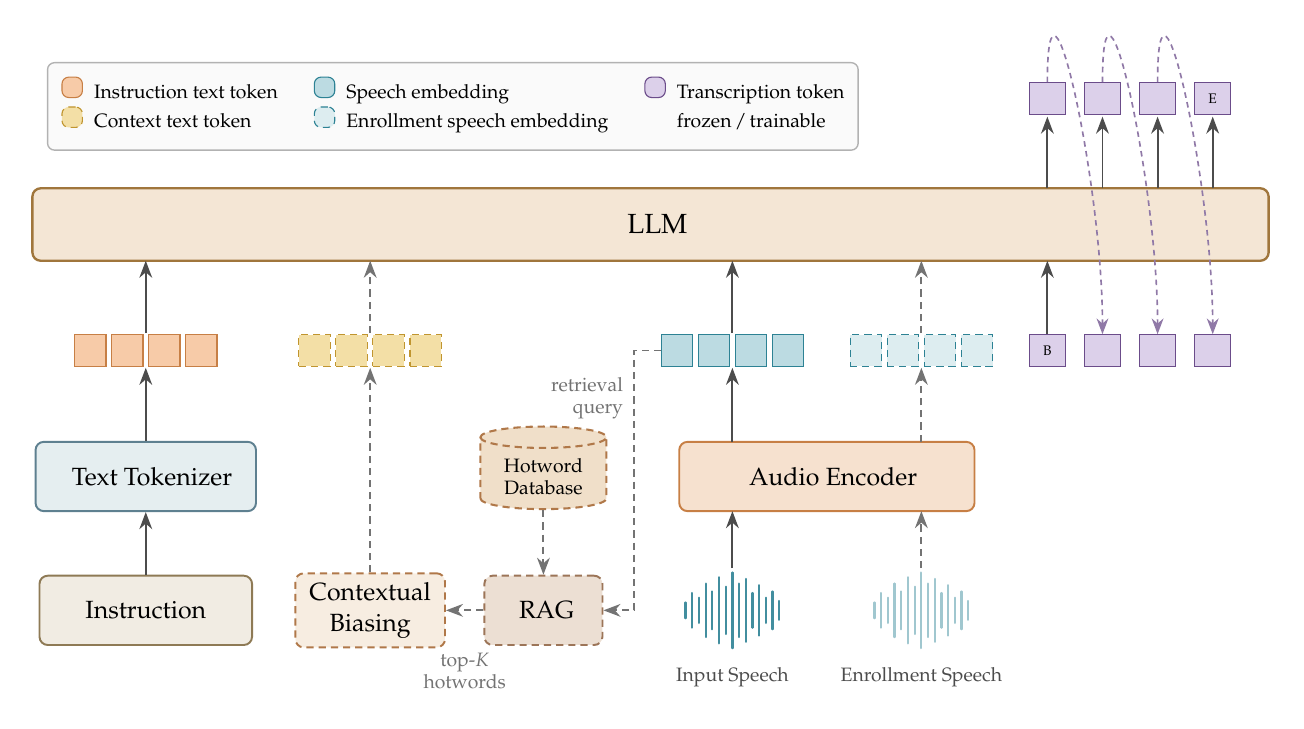
\begin{tikzpicture}
  % the feedback arcs are Bezier curves whose control points sit far above
  % the drawing, so pin the bounding box to the visible extent
  \path[use as bounding box] (-9.15, -0.90) rectangle (6.70, 7.65);

  % ===== input row =====================================================
  \node[promptbox] (instr) at (-7.65, 0.25) {Instruction};
  \node[biasbox]   (bias)  at (-4.80, 0.25) {Contextual\\Biasing};
  \node[ragbox]    (rag)   at (-2.60, 0.25) {\fireIcon~RAG};
  \node[inner sep=1pt] (src)    at (-0.20, 0.25) {\Waveform{cEncB!90}};
  \node[inner sep=1pt] (enroll) at ( 2.20, 0.25) {\Waveform{cEncB!45}};
  \node[caplabel, below=2pt of src]    {Input Speech};
  \node[caplabel, below=2pt of enroll] {Enrollment Speech};

  % ===== module row ====================================================
  \node[tokenizer] (tok)   at (-7.65, 1.95) {\frozenIcon~~Text Tokenizer};
  \node[hpool]     (hpool) at (-2.60, 1.95) {Hotword\\Database};
  \node[encoder]   (aut)   at ( 1.00, 1.95) {\fireIcon~~Audio Encoder};

  % retrieval chain: the database sits right above RAG, so its arrow lands
  % on the RAG centre; the hotwords leave horizontally to the left
  \draw[dashedflow] (hpool.south) -- (rag.north);
  \draw[dashedflow] (rag.west) -- (bias.east);
  \node[edgelabel, align=center] at (-3.60, -0.52) {top-$K$\\hotwords};

  % instruction -> tokenizer; the two encoder inputs are equal-length
  % verticals placed symmetrically about the encoder centre
  \draw[flow]       (instr.north)  -- (tok.south);
  \draw[flow]       (src.north)    -- (-0.20, 1.51);
  \draw[dashedflow] (enroll.north) -- ( 2.20, 1.51);

  % ===== token row =====================================================
  \foreach \gx/\st in {-7.650/cellIns, -4.800/cellCtx,
                       -0.200/cellSpc,  2.200/cellEnr}{
    \foreach \i in {0,1,2,3}{
      \pgfmathsetmacro{\xc}{\gx + (\i-1.5)*0.47}
      \node[\st] at (\xc, 3.55) {};
    }
  }

  % every group is fed by a single straight vertical; the encoder's two
  % outputs are symmetric about its centre and therefore equal in length
  \draw[flow]       (tok.north)  -- (-7.650, 3.33);
  \draw[dashedflow] (bias.north) -- (-4.800, 3.33);
  \draw[flow]       (-0.200, 2.39) -- (-0.200, 3.33);
  \draw[dashedflow] ( 2.200, 2.39) -- ( 2.200, 3.33);

  % the encoded speech itself is the retrieval query: it leaves the speech
  % embeddings sideways and enters RAG from the right, on the same line as
  % the hotwords leaving on the left
  \draw[dashedflow] (-1.105, 3.55) -- (-1.450, 3.55) -- (-1.450, 0.25)
                    -- (rag.east);
  \node[edgelabel, anchor=east, align=right] at (-1.53, 2.95)
        {retrieval\\query};

  % ===== LLM ===========================================================
  \node[llmbox] (llm) at (-1.24, 5.15) {\fireIcon~~LLM};

  \draw[flow]       (-7.650, 3.77) -- (-7.650, 4.69);
  \draw[dashedflow] (-4.800, 3.77) -- (-4.800, 4.69);
  \draw[flow]       (-0.200, 3.77) -- (-0.200, 4.69);
  \draw[dashedflow] ( 2.200, 3.77) -- ( 2.200, 4.69);

  % ===== autoregressive decoding =======================================
  % each emitted token re-enters the sequence as the input of the next step
  \node[cellOut, font=\tiny] (p0) at (3.80, 3.55) {B};
  \node[cellOut]             (p1) at (4.50, 3.55) {};
  \node[cellOut]             (p2) at (5.20, 3.55) {};
  \node[cellOut]             (p3) at (5.90, 3.55) {};

  \node[cellOut]             (q0) at (3.80, 6.75) {};
  \node[cellOut]             (q1) at (4.50, 6.75) {};
  \node[cellOut]             (q2) at (5.20, 6.75) {};
  \node[cellOut, font=\tiny] (q3) at (5.90, 6.75) {E};

  \draw[flow] (p0.north) -- (3.80, 4.69);
  \foreach \x in {3.80, 4.50, 5.20, 5.90}{
    \draw[flow] (\x, 5.61) -- (\x, 6.52);
  }
  \draw[arcflow] (q0.north) to[out=90, in=90, looseness=1.5] (p1.north);
  \draw[arcflow] (q1.north) to[out=90, in=90, looseness=1.5] (p2.north);
  \draw[arcflow] (q2.north) to[out=90, in=90, looseness=1.5] (p3.north);

  % ===== legend (top-left, one entry per token type) ===================
  \node[draw=black!30, rounded corners=2.5pt, fill=black!2,
        line width=0.5pt, align=left, inner sep=5pt] at (-3.75, 6.65) {%
    \scriptsize
    \renewcommand{\arraystretch}{1.25}%
    \begin{tabular}{@{}c@{\hspace{4pt}}l@{\hspace{13pt}}c@{\hspace{4pt}}l@{\hspace{13pt}}c@{\hspace{4pt}}l@{}}
      \tikz\node[cellIns, legcell]{}; & Instruction text token &
      \tikz\node[cellSpc, legcell]{}; & Speech embedding &
      \tikz\node[cellOut, legcell]{}; & Transcription token\\
      \tikz\node[cellCtx, legcell]{}; & Context text token &
      \tikz\node[cellEnr, legcell]{}; & Enrollment speech embedding &
      \frozenIcon~\fireIcon & frozen\,/\,trainable\\
    \end{tabular}%
  };

\end{tikzpicture}
\end{document}
